\documentclass[11pt,a4paper]{article}
%%%%%%%%%%%%%%%%%%%%%%%%% Credit %%%%%%%%%%%%%%%%%%%%%%%%

% template ini dibuat oleh martin.manullang@if.itera.ac.id untuk dipergunakan oleh seluruh sivitas akademik itera.

%%%%%%%%%%%%%%%%%%%%%%%%% PACKAGE starts HERE %%%%%%%%%%%%%%%%%%%%%%%%
\usepackage{graphicx}
\usepackage{caption}
\usepackage{microtype}
\captionsetup[table]{name=Tabel}
\captionsetup[figure]{name=Gambar}
\usepackage{tabulary}
\usepackage{minted}
\usepackage{fancyhdr}
\usepackage{placeins}
\usepackage{graphicx}
\usepackage[all]{xy}
\usepackage{tikz}
\usepackage{verbatim}
\usepackage[left=2cm,right=2cm,top=3cm,bottom=2.5cm]{geometry}
\usepackage{hyperref}
\hypersetup{
    colorlinks,
    linkcolor={red!50!black},
    citecolor={blue!50!black},
    urlcolor={blue!80!black}
}
\usepackage{caption}
\usepackage{subcaption}
\usepackage{multirow}
\usepackage{psfrag}
\usepackage[T1]{fontenc}
\usepackage[scaled]{beramono}
\usepackage{listings}
\usepackage{xcolor} 
% custom color & style for listing
\definecolor{codegreen}{rgb}{0,0.6,0}
\definecolor{codegray}{rgb}{0.5,0.5,0.5}
\definecolor{codepurple}{rgb}{0.58,0,0.82}
\definecolor{backcolour}{rgb}{0.95,0.95,0.92}
\definecolor{LightGray}{gray}{0.9}
\lstdefinestyle{mystyle}{
    backgroundcolor=\color{backcolour},   
    commentstyle=\color{green},
    keywordstyle=\color{codegreen},
    numberstyle=\tiny\color{codegray},
    stringstyle=\color{codepurple},
    basicstyle=\ttfamily\footnotesize,
    breakatwhitespace=false,         
    breaklines=true,                 
    captionpos=b,                    
    keepspaces=true,                 
    numbers=left,                    
    numbersep=5pt,                  
    showspaces=false,                
    showstringspaces=false,
    showtabs=false,                  
    tabsize=2
}
\lstset{style=mystyle}
\renewcommand{\lstlistingname}{Kode}
%%%%%%%%%%%%%%%%%%%%%%%%% PACKAGE ends HERE %%%%%%%%%%%%%%%%%%%%%%%%

%%%%%%%%%%%%%%%%%%%%%%%%% Data Diri %%%%%%%%%%%%%%%%%%%%%%%%
\newcommand{\studentone}{Muhamad Ivan Aulia Rahman}
\newcommand{\studenttwo}{Nasrul Alfin Prassetyo}
\newcommand{\studentthree}{Muhammad Faisal Safira}
\newcommand{\course}{Tugas Besar Multimedia (IF4021)}
\newcommand{\assignment}{Filter Truth or Dare}

%%%%%%%%%%%%%%%%%%% using theorem style %%%%%%%%%%%%%%%%%%%%
\newtheorem{thm}{Theorem}
\newtheorem{lem}[thm]{Lemma}
\newtheorem{defn}[thm]{Definition}
\newtheorem{exa}[thm]{Example}
\newtheorem{rem}[thm]{Remark}
\newtheorem{coro}[thm]{Corollary}
\newtheorem{quest}{Question}[section]
%%%%%%%%%%%%%%%%%%%%%%%%%%%%%%%%%%%%%%%%
\usepackage{lipsum}
\usepackage{fancyhdr}
\pagestyle{fancy}
\lhead{Muhamad Ivan Aulia Rahman, Nasrul Alfin Prassetyo, Muhammad Faisal Safira}
\rhead{ \thepage}
\cfoot{Filter Truth or Dare}
\renewcommand{\headrulewidth}{0.4pt}
\renewcommand{\footrulewidth}{0.4pt}
\setlength\headheight{14pt}

\begin{document}
\thispagestyle{empty}
\begin{center}
    \includegraphics[scale = 0.15]{Figure/ifitera-header.png}
    \vspace{0.1cm}
\end{center}
\noindent
\rule{17cm}{0.2cm}\\[0.3cm]
Anggota 1: \studentone \hfill Judul Tugas: \assignment\\[0.1cm]
Anggota 2: \studenttwo \hfill Tanggal: 20 Desember 2024\\[0.1cm]
Anggota 3: \studentthree \hfill\\[0.1cm]
Mata Kuliah: \course \hfill\\[0.1cm]
\rule{17cm}{0.05cm}
\vspace{0.1cm}

\section*{Abstrak}
Filter Truth or Dare adalah program sederhana yang dikembangkan menggunakan bahasa pemrograman Python. Program ini dirancang untuk memberikan pengalaman interaktif dalam permainan Truth or Dare dengan memilih secara acak antara dua opsi: "Truth" (kejujuran) atau "Dare" (tantangan). Dengan menggunakan daftar pertanyaan dan tantangan yang telah disiapkan, program ini dapat memberikan pertanyaan yang menarik atau tantangan yang menghibur kepada pengguna. Melalui interaksi yang mudah dan menyenangkan, program ini bertujuan untuk meningkatkan pengalaman bermain dan mempererat hubungan antar peserta.

\textbf{Kata Kunci}: Interaksi Pengguna, Pengalaman Bermain, Program Python.

\newpage

\tableofcontents
\newpage

\section{Pendahuluan}
\subsection{Latar Belakang Masalah}

Media sosial, terutama aplikasi seperti TikTok, telah menjadi fenomena global yang mengubah cara orang berinteraksi dan berbagi konten. TikTok memungkinkan pengguna untuk membuat video pendek yang kreatif, sering kali berisi tantangan dan permainan, yang menarik perhatian banyak orang, terutama di kalangan remaja. Dengan fitur-fitur yang menarik, TikTok tidak hanya menjadi sarana hiburan, tetapi juga platform untuk mengekspresikan diri dan berinteraksi dengan orang lain.

Namun, di balik popularitasnya, terdapat kekhawatiran mengenai dampak penggunaan aplikasi ini terhadap perilaku sosial dan psikologis penggunanya. Penggunaan yang berlebihan dapat menyebabkan kecanduan, mempengaruhi pola pikir, dan mengubah cara individu berinteraksi dalam kehidupan sehari-hari. Oleh karena itu, penting untuk memahami efek dari aplikasi ini dan bagaimana program seperti "Filter Truth or Dare" dapat memberikan pengalaman interaktif yang positif dalam konteks permainan sosial.


\subsection{Rumusan Masalah}
\begin{enumerate}
    \item Bagaimana program "Filter Truth or Dare" dapat meningkatkan interaksi sosial pengguna dalam konteks permainan?
    \item Bagaimana efektivitas penggunaan teknologi pelacakan wajah dalam meningkatkan pengalaman bermain?
\end{enumerate}

\subsection{Tujuan Penelitian}
\begin{enumerate}
    \item Mengembangkan program interaktif "Filter Truth or Dare" untuk meningkatkan pengalaman bermain dan interaksi sosial pengguna.
    \item Mengevaluasi efektivitas teknologi pelacakan wajah dalam mendukung permainan interaktif.
    \item Memberikan rekomendasi pengembangan lebih lanjut untuk aplikasi berbasis interaksi sosial.
\end{enumerate}

\subsection{Batasan Masalah}
\begin{enumerate}
    \item Penelitian ini akan dibatasi pada pengguna TikTok yang berusia antara 13 hingga 19 tahun, mengingat kelompok usia ini merupakan mayoritas pengguna aktif aplikasi tersebut.
    \item Penelitian akan berfokus pada dampak sosial dan psikologis dari penggunaan TikTok, termasuk perubahan dalam interaksi sosial, pola pikir, dan perilaku pengguna.
\end{enumerate}

\subsection{Manfaat Penelitian}
\begin{enumerate}
    \item Penelitian ini dapat memberikan kontribusi dalam pengembangan program interaktif seperti "Filter Truth or Dare" yang dapat meningkatkan interaksi sosial positif di kalangan remaja, serta memberikan alternatif hiburan yang lebih konstruktif.
    \item Penelitian ini diharapkan dapat memberikan pemahaman yang lebih mendalam tentang dampak penggunaan TikTok terhadap perilaku sosial dan psikologis remaja, sehingga dapat membantu orang tua, pendidik, dan pembuat kebijakan dalam memahami fenomena ini.
\end{enumerate}

\newpage
\section{Tinjauan Pustaka}
\subsection{Face Tracking}
Face tracking adalah teknologi yang digunakan untuk mendeteksi dan mengikuti posisi wajah dalam gambar atau video. Teknologi ini sering kali menggunakan algoritma berbasis machine learning, seperti Convolutional Neural Networks (CNN), untuk meningkatkan akurasi deteksi wajah dalam berbagai kondisi. Face tracking memungkinkan aplikasi untuk memberikan efek visual yang responsif terhadap gerakan wajah pengguna, sehingga menciptakan pengalaman interaktif yang lebih menarik. Menurut [1], teknik pelacakan wajah yang efektif sangat penting dalam aplikasi multimedia untuk meningkatkan keterlibatan pengguna.

\subsection{Python}
Python adalah bahasa pemrograman yang populer dan banyak digunakan dalam pengembangan aplikasi multimedia, termasuk aplikasi yang memanfaatkan teknologi pelacakan wajah dan Augmented Reality. Python memiliki berbagai pustaka (library) yang mendukung pengolahan citra dan machine learning, seperti OpenCV dan TensorFlow. Dengan kemudahan sintaksis dan fleksibilitasnya, Python memungkinkan pengembang untuk dengan cepat mengimplementasikan algoritma pelacakan wajah dan mengintegrasikannya ke dalam aplikasi interaktif. Menurut van Rossum dan Drake [4], Python adalah pilihan yang ideal untuk pengembangan prototipe dan aplikasi multimedia.

\subsection{Truth or Dare}
Truth or Dare adalah permainan sosial yang melibatkan dua pilihan: menjawab pertanyaan jujur atau melakukan tantangan. Permainan ini sering dimainkan dalam kelompok dan dapat meningkatkan interaksi sosial di antara peserta. Dalam konteks aplikasi interaktif, permainan ini dapat diadaptasi dengan menambahkan elemen digital, seperti filter wajah, untuk meningkatkan pengalaman bermain. Menurut Kim [3], permainan interaktif yang melibatkan elemen sosial dapat memperkuat hubungan antar individu dan menciptakan suasana yang menyenangkan.

\newpage
\section{Metode Penelitian}
\subsection{Alur Penelitian}

\begin{enumerate}
    \item Identifikasi Masalah

    Pada penelitian ini, masalah utama yang diidentifikasi adalah bagaimana menciptakan filter interaktif berbasis permainan Truth or Dare yang dapat meningkatkan pengalaman bermain melalui teknologi deteksi wajah. Permainan Truth or Dare tradisional sering kali bergantung pada interaksi sosial langsung, namun dengan berkembangnya teknologi, ada kebutuhan untuk menciptakan pengalaman yang lebih dinamis dan menyenangkan, khususnya bagi pemain yang menginginkan pengalaman yang lebih interaktif dan berbasis teknologi. Salah satu tantangan yang perlu dipecahkan adalah bagaimana mendeteksi gerakan atau arah kepala pemain dengan akurat menggunakan teknologi deteksi wajah, serta bagaimana memanfaatkan deteksi tersebut untuk memicu aksi dalam permainan, seperti memilih antara Truth atau Dare. Selain itu, diperlukan integrasi antara pemrosesan visual, efek suara, dan tampilan antarmuka yang intuitif agar permainan dapat berjalan dengan lancar dan memberikan hiburan yang maksimal.
    \item Kajian Pustaka

    Kajian pustaka dalam penelitian ini mencakup berbagai topik yang relevan untuk pengembangan filter interaktif berbasis permainan Truth or Dare. Pertama, teknologi deteksi wajah menjadi elemen utama dalam menciptakan pengalaman interaktif. MediaPipe, yang dikembangkan oleh Google, adalah salah satu library yang populer untuk deteksi wajah dan pelacakan gerakan, yang memungkinkan pengenalan wajah secara real-time. Berdasarkan beberapa penelitian, MediaPipe telah terbukti efektif dalam mendeteksi wajah dengan akurasi tinggi dan kecepatan pemrosesan yang baik, sehingga sangat cocok digunakan dalam aplikasi permainan interaktif seperti ini. Selain itu, kajian terkait implementasi game-based learning dan aplikasi permainan berbasis teknologi juga mendukung pentingnya elemen interaktif dalam meningkatkan keterlibatan pemain. Dalam konteks ini, penggunaan efek visual dan audio untuk meningkatkan pengalaman pengguna juga mendapatkan perhatian, di mana efek visual seperti gradient overlay dan pengaturan audio berbasis pilihan permainan dapat menciptakan atmosfer yang lebih menarik. Beberapa studi sebelumnya menunjukkan bahwa efek-efek ini dapat meningkatkan pengalaman pengguna dan memberikan elemen kejutan serta hiburan.
    \item Perancangan Sistem

    Perancangan sistem dilakukan dengan mengembangkan filter interaktif berbasis permainan Truth or Dare dengan teknologi deteksi wajah. Sistem ini terdiri dari beberapa komponen utama yang bekerja secara terintegrasi untuk menciptakan pengalaman bermain yang dinamis dan interaktif. Pertama, sistem akan menggunakan kamera untuk menangkap gambar atau video dari pemain, yang kemudian dianalisis menggunakan algoritma deteksi wajah berbasis MediaPipe. Berdasarkan posisi dan arah wajah, sistem akan menentukan gerakan kepala pemain, apakah mengarah ke kiri, kanan, atau berada di posisi netral. Pemain yang menggerakkan kepala ke kiri akan dipilihkan Truth, sedangkan ke kanan akan dipilihkan Dare, sementara posisi netral akan memicu pemilihan acak antara keduanya. Selanjutnya, sistem akan menampilkan pertanyaan atau tantangan sesuai pilihan, dengan efek visual seperti gradient overlay yang disesuaikan dengan pilihan pemain, serta efek audio untuk menambah kesan interaktif. Selain itu, sistem juga dilengkapi dengan fitur countdown timer untuk memberikan ketegangan pada permainan. Untuk memastikan kenyamanan pengguna, desain antarmuka yang sederhana dan responsif akan diterapkan, sehingga pemain dapat berfokus pada permainan tanpa gangguan. Dengan perancangan ini, sistem diharapkan dapat memberikan hiburan yang lebih menarik dan meningkatkan keterlibatan pemain dalam permainan Truth or Dare.
    \item Pengujian Sistem

    Pengujian sistem bertujuan untuk memastikan bahwa seluruh komponen yang dirancang berfungsi dengan baik dan sesuai dengan tujuan yang diinginkan. Pengujian pertama akan dilakukan untuk mengevaluasi akurasi deteksi wajah dan arah kepala menggunakan algoritma MediaPipe. Uji coba akan melibatkan beberapa kondisi, seperti variasi posisi wajah, pencahayaan, dan gerakan kepala, untuk memastikan sistem dapat mendeteksi arah kepala secara tepat dan responsif. Selanjutnya, pengujian dilakukan pada sistem pemilihan Truth atau Dare berdasarkan arah kepala dan pemilihan acak jika kepala berada dalam posisi netral. Pengujian terhadap integrasi efek visual dan audio juga penting untuk memastikan bahwa efek seperti gradient overlay dan suara latar berfungsi dengan baik, memberikan umpan balik yang sesuai dengan pilihan pemain. Selain itu, sistem akan diuji dengan melibatkan beberapa pengguna untuk mendapatkan umpan balik mengenai responsivitas dan kenyamanan antarmuka, serta kesesuaian pengalaman bermain dengan ekspektasi pemain. Selama pengujian, dilakukan analisis terhadap kecepatan pemrosesan, kestabilan aplikasi, serta pengalaman pengguna secara keseluruhan. Hasil pengujian akan digunakan untuk melakukan perbaikan dan optimasi agar sistem dapat berjalan dengan lebih efektif
    \item Analisis dan Evaluasi

    Analisis dan evaluasi sistem dilakukan untuk mengukur sejauh mana sistem yang dikembangkan memenuhi tujuan yang telah ditetapkan dalam penelitian ini. Pertama, evaluasi dilakukan terhadap akurasi dan kecepatan deteksi arah kepala menggunakan algoritma MediaPipe. Hasil analisis akan menunjukkan tingkat ketepatan sistem dalam mendeteksi posisi kepala pemain, serta responsivitas sistem terhadap gerakan yang dilakukan. Selanjutnya, efektivitas mekanisme pemilihan Truth atau Dare berdasarkan arah kepala akan dianalisis dengan memeriksa apakah sistem dapat secara konsisten memicu pilihan yang tepat sesuai dengan pergerakan kepala pemain. Evaluasi juga mencakup pengujian terhadap kualitas efek visual dan audio yang diterapkan, serta pengaruhnya terhadap pengalaman pengguna. Dengan melakukan analisis terhadap feedback pengguna, kami akan mengidentifikasi area yang perlu diperbaiki, seperti peningkatan kecepatan pemrosesan atau peningkatan responsivitas antarmuka pengguna.
\end{enumerate}

\newpage
\section{Hasil dan Pembahasan}
\subsection{Pembahasan}
\begin{figure}[H]
    \centering
    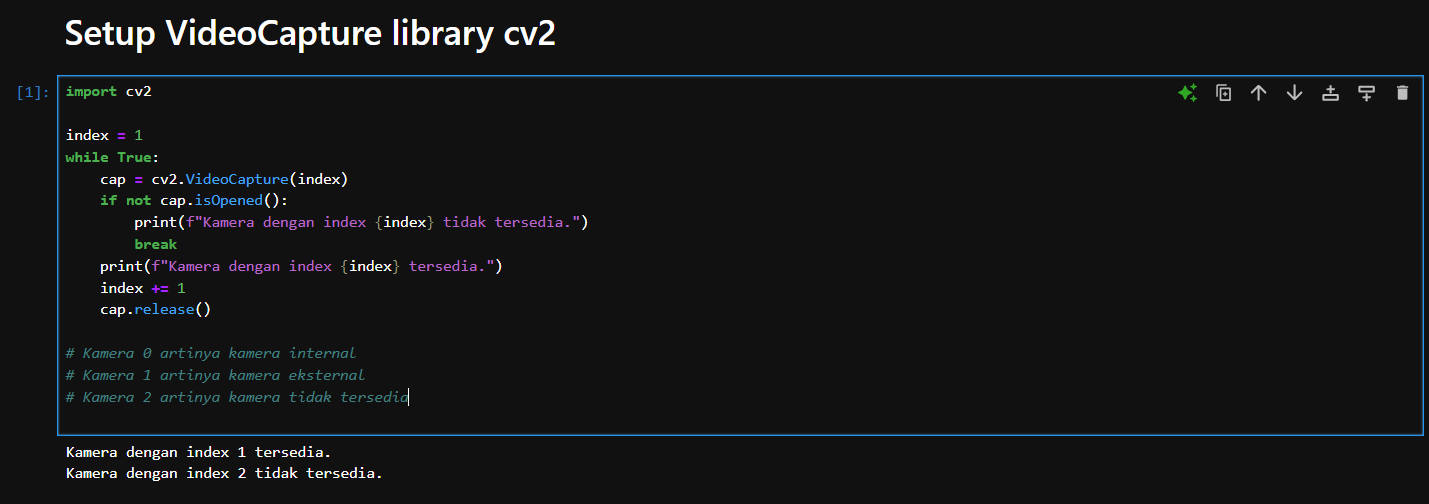
\includegraphics[width=0.8\textwidth]{1.png} % Sesuaikan nama file gambar
    \caption{Kode Program 1}
    \label{fig:1}
\end{figure}
\textbf{Penjelasan Program:}
\begin{enumerate}
    \item \textbf{cv2.VideoCapture(index)}: Digunakan untuk mencoba membuka kamera berdasarkan indeks yang diberikan ( 0 untuk kamera internal dan 1 untuk kamera eksternal).
    \item \textbf{cap.isOpened()}: Mengecek apakah kamera berhasil dibuka. Jika berhasil, maka kamera tersebut tersedia.
    \item \textbf{cap.release()}: Menutup akses ke kamera setelah selesai digunakan.
    \item \textbf{index += 1}: Meningkatkan nilai indeks untuk mencoba membuka kamera berikutnya, hingga kamera yang dimaksud tidak tersedia.
\end{enumerate}

\textbf{Alur Program:}
\begin{enumerate}
    \item \textbf{Kamera dengan index 0} merujuk ke kamera internal laptop atau komputer.
    \item \textbf{Kamera dengan index 1} ke kamera eksternal, seperti webcam yang terhubung.
    \item \textbf{Kamera dengan index 2} dan seterusnya digunakan untuk kamera lain yang mungkin terhubung ke sistem.
\end{enumerate}

\begin{figure}[H]
    \centering
    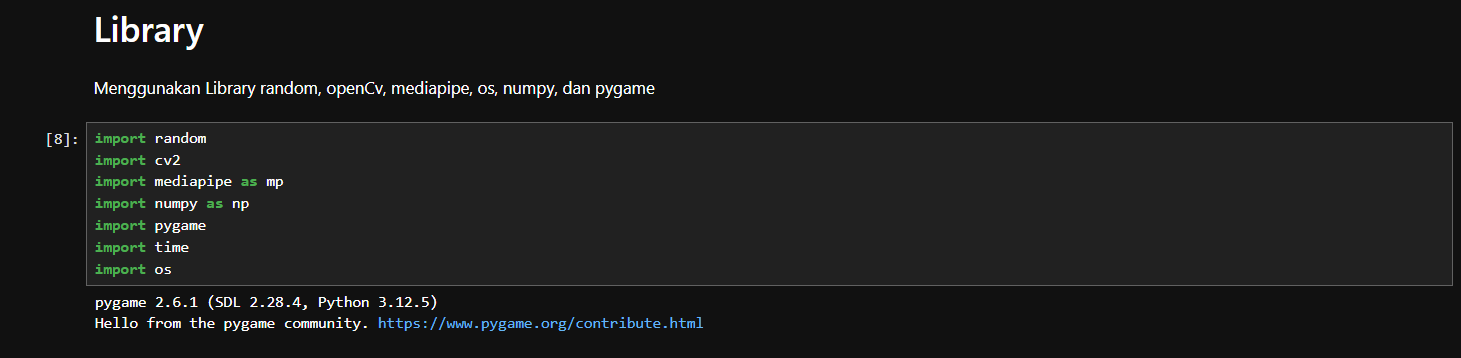
\includegraphics[width=0.8\textwidth]{2.png} % Sesuaikan nama file gambar
    \caption{Kode Program 2}
    \label{fig:2}
\end{figure}

\begin{enumerate}
    \item \textbf{import random}
    
Digunakan untuk menghasilkan angka acak. Dalam konteks permainan, ini dapat digunakan untuk memilih pertanyaan Truth atau Dare secara acak atau untuk memilih dari opsi yang tersedia.
    \item \textbf{import cv2}
    
OpenCV (Open Source Computer Vision Library) digunakan untuk memproses gambar dan video. Di sini, OpenCV akan digunakan untuk menangkap video dari kamera, memproses gambar real-time, dan menampilkan hasil deteksi wajah.
    \item \textbf{import mediapipe as mp}
    
MediaPipe adalah framework dari Google untuk deteksi objek, termasuk deteksi wajah, pose tubuh, tangan, dll. Di program Anda, MediaPipe digunakan untuk mendeteksi gerakan kepala dan wajah secara real-time untuk mengontrol permainan.
    \item \textbf{import numpy as np}
    
NumPy adalah library untuk komputasi numerik di Python. Ini sering digunakan untuk manipulasi array dan matriks, serta untuk menghitung berbagai parameter dalam pengolahan gambar ( piksel gambar).
    \item \textbf{import pygame}
    
Pygame adalah library untuk membuat aplikasi grafis dan game. Di program Anda, Pygame kemungkinan digunakan untuk menampilkan antarmuka pengguna (UI) atau suara dan efek visual dalam permainan Truth or Dare.
    \item \textbf{import time}
    
Library ini menyediakan fungsi untuk mengontrol waktu, misalnya untuk menunda eksekusi program atau untuk menghitung durasi antara tindakan, seperti delay antara pertanyaan atau tantangan dalam permainan.
    \item \textbf{import os}
    
os digunakan untuk berinteraksi dengan sistem operasi, misalnya untuk menangani file, direktori, atau menjalankan perintah sistem. Digunakan untuk memanipulasi file yang diperlukan oleh permainan atau untuk mengakses data eksternal.
\end{enumerate}

\begin{figure}[H]
    \centering
    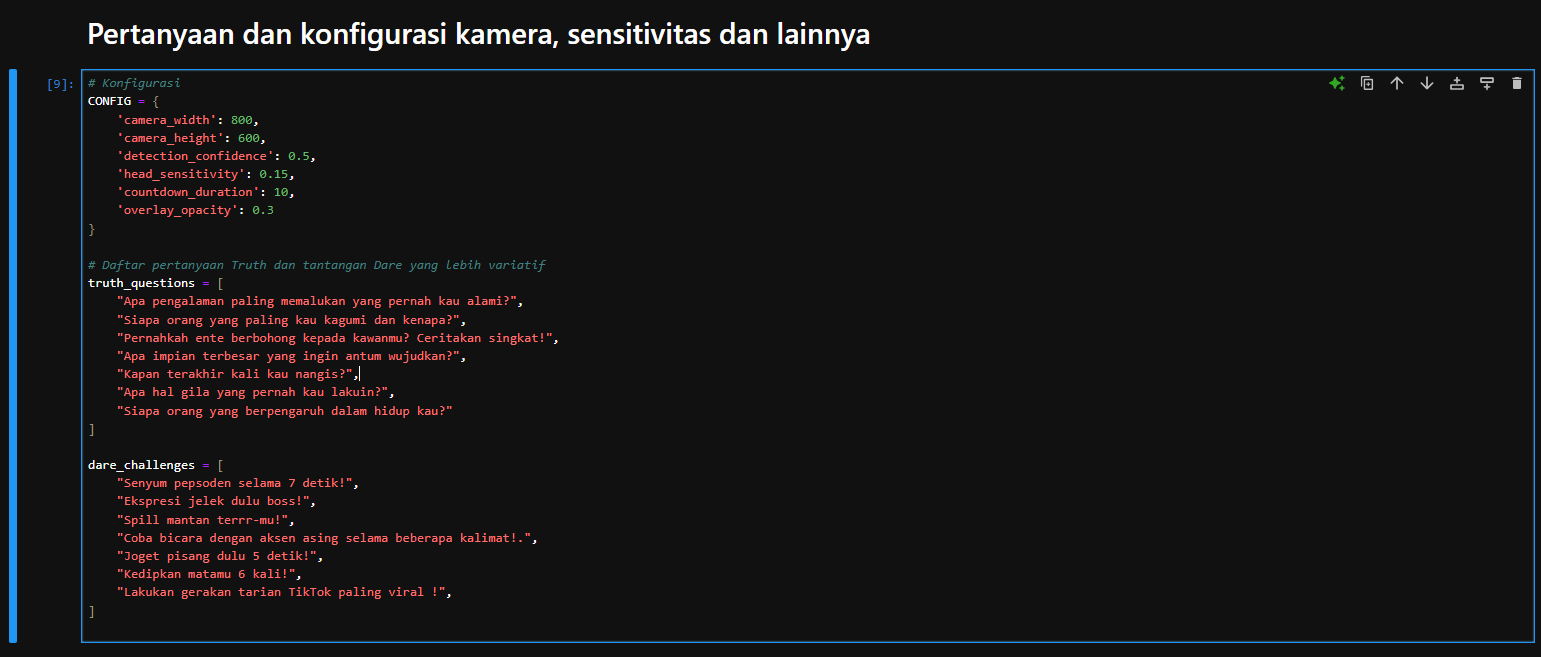
\includegraphics[width=0.8\textwidth]{3.png} % Sesuaikan nama file gambar
    \caption{Kode Program 3}
    \label{fig:3}
\end{figure}

\newpage
\textbf{Konfigurasi (CONFIG)}

CONFIG berisi parameter yang digunakan untuk mengatur berbagai aspek permainan dan pengolahan gambar:
\begin{itemize}
    \item camera\_width: Menentukan lebar tampilan kamera. Dalam hal ini, ukuran lebar kamera diatur menjadi 800 piksel.
    \item camera\_height: Menentukan tinggi tampilan kamera. Ukuran tinggi diatur menjadi 600 piksel.
    \item detection\_confidence: Menentukan tingkat kepercayaan (confidence level) dalam deteksi wajah oleh MediaPipe. Nilai 0.5 berarti deteksi akan dilakukan jika tingkat kepercayaan wajah terdeteksi mencapai setidaknya 50%.
    \item head\_sensitivity: Menentukan sensitivitas untuk mendeteksi gerakan kepala. Nilai 0.15 berarti gerakan kepala harus cukup besar agar dianggap sebagai input yang valid.
    \item countdown\_duration: Durasi hitung mundur dalam detik sebelum permainan dimulai atau saat memilih antara Truth dan Dare. Durasi ini diatur menjadi 10 detik.
    \item overlay\_opacity: Mengatur opasitas overlay di layar, untuk memberikan efek transparan pada elemen antarmuka, diatur ke 0.3 yang berarti 30% transparan.
\end{itemize}

\textbf{Daftar Pertanyaan Truth}

Ini adalah daftar pertanyaan Truth yang dapat ditanyakan kepada pemain. Pertanyaan ini dirancang untuk membuat pemain berbagi pengalaman pribadi atau cerita menarik:
\begin{enumerate}
    \item Apa pengalaman paling memalukan yang pernah kau alami?
    \item Siapa orang yang paling kau kagumi dan kenapa?
    \item Pernahkah ente berbohong kepada kawanmu? Ceritakan singkat!
    \item Apa impian terbesar yang ingin antum wujudkan?
    \item Kapan terakhir kali kau nangis?
    \item Apa hal gila yang pernah kau lakuin?
    \item Siapa orang yang berpengaruh dalam hidup kau?
\end{enumerate}

\textbf{Daftar Tantangan Dare}

Ini adalah daftar tantangan Dare yang bisa diberikan kepada pemain untuk melakukan tindakan tertentu. Tantangan ini dapat membuat permainan menjadi lebih menyenangkan dan interaktif:
\begin{enumerate}
    \item Senyum pepsoden selama 7 detik!
    \item Ekspresi jelek dulu boss!
    \item Spill mantan terrr-mu!
    \item Coba bicara dengan aksen asing selama beberapa kalimat!
    \item Joget pisang dulu 5 detik!
    \item Kedipkan matamu 6 kali!
    \item Lakukan gerakan tarian TikTok paling viral!
\end{enumerate}

\newpage
\textbf{Penggunaan dalam Program}
\begin{itemize}
    \item Truth dan Dare: Ketika pemain memilih Truth atau Dare, permainan akan memilih secara acak dari masing-masing daftar ini dan menampilkan pertanyaan atau tantangan yang sesuai.
    \item Konfigurasi: Parameter dalam CONFIG digunakan untuk mengatur pengolahan gambar, durasi, dan pengaturan tampilan antarmuka untuk pengalaman bermain yang lebih nyaman dan interaktif.
\end{itemize}

\begin{figure}[H]
    \centering
    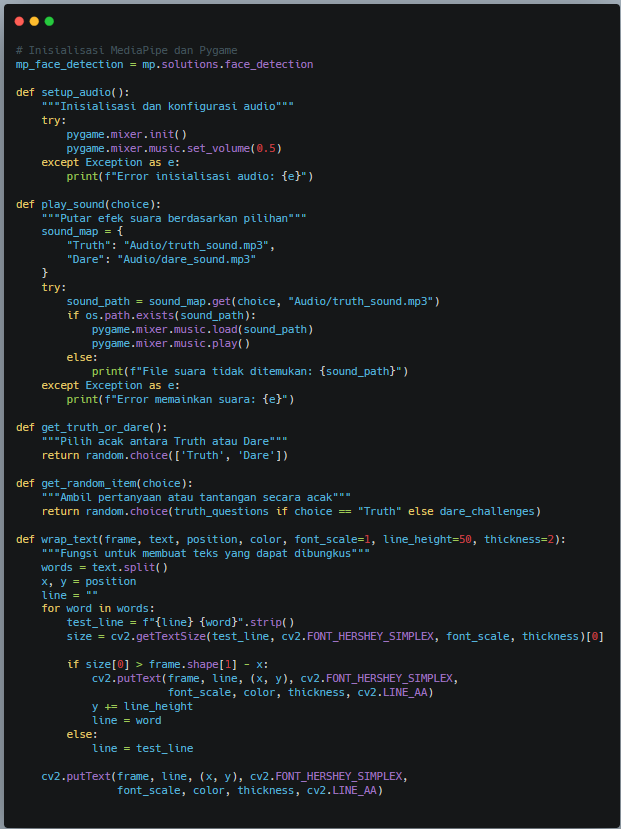
\includegraphics[width=0.8\textwidth]{4.png} % Sesuaikan nama file gambar
    \caption{Kode Program 4}
    \label{fig:4}
\end{figure}

mengonfigurasi MediaPipe, Pygame, serta beberapa fungsi tambahan untuk meningkatkan interaktivitas permainan Truth or Dare berbasis deteksi wajah dan gerakan kepala. Berikut penjelasan tentang fungsionalitas masing-masing bagian:

\textbf{Inisialisasi MediaPipe}
\begin{itemize}
    \item \textbf{mp\_face\_detection = mp.solutions.face\_detection:}

    Menyediakan akses ke model deteksi wajah yang disediakan oleh MediaPipe. Ini akan digunakan untuk mendeteksi wajah pemain dan melacak gerakan kepala mereka untuk kontrol permainan.
\end{itemize}


\textbf{Fungsi setup\_audio}
\begin{itemize}
    \item Fungsi ini menginisialisasi dan mengonfigurasi Pygame untuk memainkan efek suara. Dengan menggunakan pygame.mixer.init(), Anda memulai sistem audio dan mengatur volume suara menjadi 50% (0.5).
    \item Jika ada masalah saat menginisialisasi audio (misalnya jika tidak ada perangkat audio yang terhubung), program akan mencetak pesan kesalahan.
\end{itemize}

\textbf{Fungsi play\_sound}
\begin{itemize}
    \item \textbf{play\_sound(choice)} digunakan untuk memutar efek suara berdasarkan pilihan pemain (Truth atau Dare).
    \item \textbf{sound\_map} adalah kamus yang menghubungkan pilihan "Truth" dan "Dare" dengan file suara yang sesuai.
    \begin{itemize}
        \item Jika pemain memilih "Truth", maka \textbf{"Audio/truth\_sound.mp3"} akan diputar.
        \item Jika pemain memilih "Dare", maka "Audio/dare\_sound.mp3" akan diputar.
    \end{itemize}
    \item Fungsi ini memeriksa apakah file suara ada sebelum mencoba memutarnya. Jika file tidak ditemukan, maka akan mencetak pesan kesalahan.
\end{itemize}

\textbf{Fungsi get\_truth\_or\_dare}
\begin{itemize}
    \item Fungsi ini mengembalikan nilai acak antara "Truth" atau "Dare" dengan menggunakan \textbf{random.choice()}. Fungsi ini digunakan untuk memilih secara acak antara dua pilihan permainan.
\end{itemize}

\textbf{Fungsi get\_random\_item}
get\_random\_item(choice) memilih secara acak sebuah item dari daftar pertanyaan Truth atau tantangan Dare berdasarkan pilihan yang diberikan.
Jika pemain memilih "Truth", maka pertanyaan acak dari truth\_questions akan dikembalikan.
Jika pemain memilih "Dare", maka tantangan acak dari dare\_challenges akan dikembalikan.

\textbf{Fungsi wrap\_text}
Fungsi ini digunakan untuk menampilkan teks dalam beberapa baris, sehingga teks yang lebih panjang bisa dibungkus sesuai dengan lebar layar (frame).
\begin{itemize}
    \item frame: Frame gambar tempat teks akan ditulis (gambar video dari kamera).
    \item text: Teks yang akan ditampilkan.
    \item position: Posisi awal teks (koordinat x, y).
    \item color: Warna teks yang akan ditampilkan.
    \item font\_scale: Skala ukuran font.
    \item line\_height: Jarak vertikal antara baris teks.
    \item thickness: Ketebalan garis teks.
\end{itemize}
Fungsi ini sangat berguna untuk menampilkan teks yang lebih panjang di layar, dengan cara membungkusnya (word wrapping) dan menyesuaikan tampilannya agar tetap terlihat rapi tanpa keluar dari batas layar.

\textbf{Penggunaan dalam Permainan}
\begin{itemize}
    \item get\_truth\_or\_dare digunakan untuk menentukan apakah permainan memilih Truth atau Dare.
    \item get\_random\_item digunakan untuk mengambil pertanyaan Truth atau tantangan Dare secara acak.
    \item wrap\_text digunakan untuk menampilkan teks panjang (misalnya pertanyaan atau tantangan) di layar tanpa keluar dari batas tampilan.
    \item play\_sound digunakan untuk memutar efek suara yang sesuai dengan pilihan pemain.
\end{itemize}

\begin{figure}[H]
    \centering
    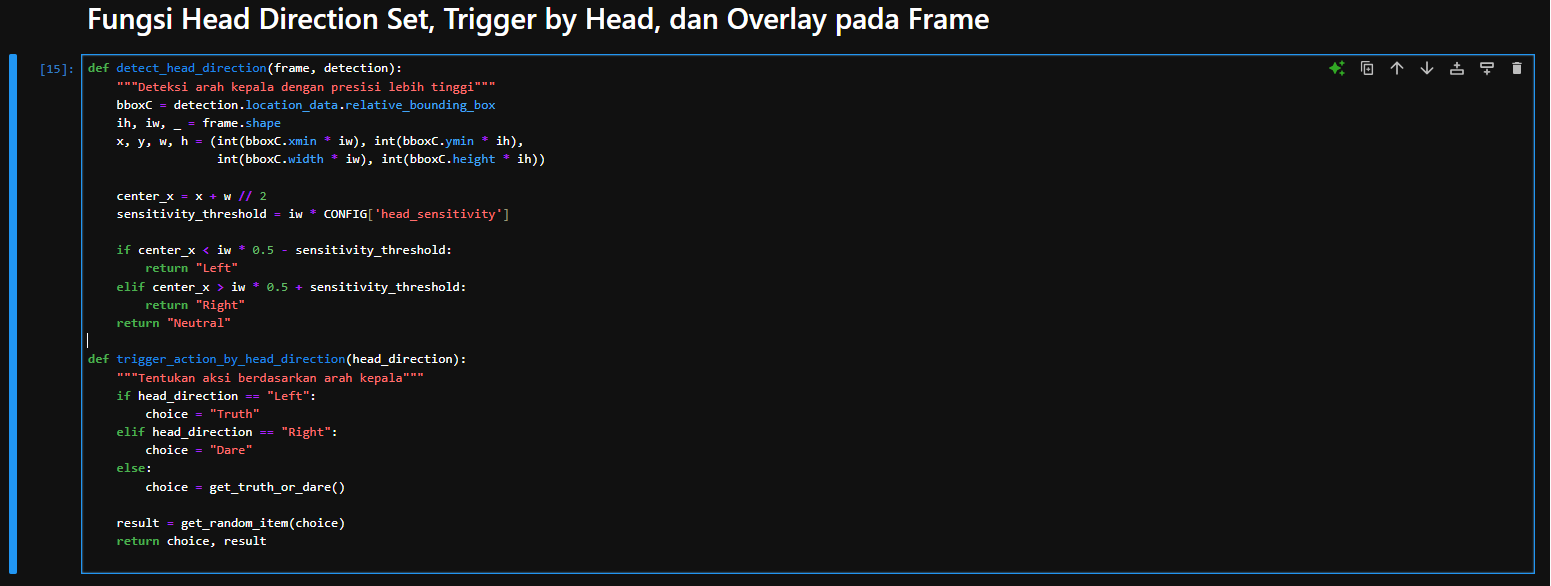
\includegraphics[width=0.8\textwidth]{5.png} % Sesuaikan nama file gambar
    \caption{Kode Program 5}
    \label{fig:5}
\end{figure}

Deteksi arah gerakan kepala dan pemicu aksi dalam permainan Truth or Dare berdasarkan arah kepala pemain. Berikut penjelasan lebih lanjut tentang masing-masing fungsi:

\textbf{Fungsi detect\_head\_direction} \\
Fungsi ini mendeteksi arah kepala pemain dengan menggunakan hasil deteksi wajah dari MediaPipe dan mengembalikan arah kepala berdasarkan posisi horizontal wajah pada frame video.

\textbf{Penjelasan:} \\
\texttt{bboxC = detection.location\_data.relative\_bounding\_box}: \\
Menangkap bounding box relatif dari wajah yang terdeteksi oleh MediaPipe. Ini berisi informasi tentang posisi dan ukuran wajah dalam bentuk koordinat relatif (berdasarkan persentase ukuran gambar).

\texttt{ih, iw, \_ = frame.shape}: \\
Menyimpan dimensi gambar (tinggi \texttt{ih} dan lebar \texttt{iw}) dari frame video.

\texttt{x, y, w, h = (int(bboxC.xmin * iw), int(bboxC.ymin * ih), int(bboxC.width * iw), int(bboxC.height * ih))}: \\
Menghitung koordinat absolut (\texttt{x, y}) dan ukuran (\texttt{w, h}) dari bounding box wajah berdasarkan dimensi frame. Ini memungkinkan untuk menggambar kotak pembatas wajah di layar.

\texttt{center\_x = x + w // 2}: \\
Menghitung koordinat pusat dari bounding box wajah (koordinat horizontal tengah wajah).

\texttt{sensitivity\_threshold = iw * CONFIG['head\_sensitivity']}: \\
Menentukan ambang batas sensitivitas berdasarkan lebar frame dan nilai sensitivitas kepala yang ditetapkan dalam konfigurasi (misalnya, 15\% dari lebar layar).

\textbf{Logika Arah Kepala:} \\
\begin{itemize}
    \item Jika posisi horizontal tengah wajah berada di kiri dari layar dengan ambang batas sensitivitas, maka arah kepala dianggap \texttt{"Left"}.
    \item Jika posisi horizontal tengah wajah berada di kanan dari layar dengan ambang batas sensitivitas, maka arah kepala dianggap \texttt{"Right"}.
    \item Jika posisi wajah berada di tengah layar (dalam rentang sensitivitas), maka arah kepala dianggap \texttt{"Neutral"}.
\end{itemize}

\textbf{Return:} \\
Fungsi ini mengembalikan satu dari tiga nilai: \texttt{"Left"}, \texttt{"Right"}, atau \texttt{"Neutral"} tergantung pada posisi wajah pemain.

\textbf{Fungsi trigger\_action\_by\_head\_direction} 

Fungsi ini memicu aksi dalam permainan berdasarkan arah kepala yang terdeteksi oleh fungsi \texttt{detect\_head\_direction}. Aksi yang diambil adalah memilih antara Truth atau Dare dan memilih pertanyaan atau tantangan acak dari daftar yang sesuai.

\textbf{Penjelasan:} \\
\begin{itemize}
    \item \texttt{if head\_direction == "Left"}: \\
    Jika arah kepala terdeteksi ke kiri, permainan akan memilih Truth untuk pemain.
    \item \texttt{elif head\_direction == "Right"}: \\
    Jika arah kepala terdeteksi ke kanan, permainan akan memilih Dare untuk pemain.
    \item \texttt{else}: \\
    Jika kepala berada dalam posisi netral (tengah), maka permainan akan memilih acak antara Truth atau Dare menggunakan fungsi \texttt{get\_truth\_or\_dare()}.
\end{itemize}

\texttt{result = get\_random\_item(choice)}: \\
Setelah menentukan pilihan Truth atau Dare, fungsi \texttt{get\_random\_item(choice)} akan dipanggil untuk mengambil pertanyaan atau tantangan acak dari daftar yang sesuai.

\textbf{Return:} \\
Fungsi ini mengembalikan dua nilai: pilihan Truth atau Dare yang dipilih dan hasil acak dari daftar pertanyaan atau tantangan.

\textbf{Penggunaan dalam Program:} \\
\begin{itemize}
    \item \texttt{detect\_head\_direction} digunakan untuk mendeteksi dan menentukan arah kepala pemain dengan presisi lebih tinggi, berdasarkan posisi wajah yang terdeteksi.
    \item \texttt{trigger\_action\_by\_head\_direction} akan menentukan apakah pemain memilih Truth atau Dare berdasarkan arah kepala mereka. Setelah itu, permainan akan memilih pertanyaan atau tantangan secara acak.
\end{itemize}

\begin{figure}[H]
    \centering
    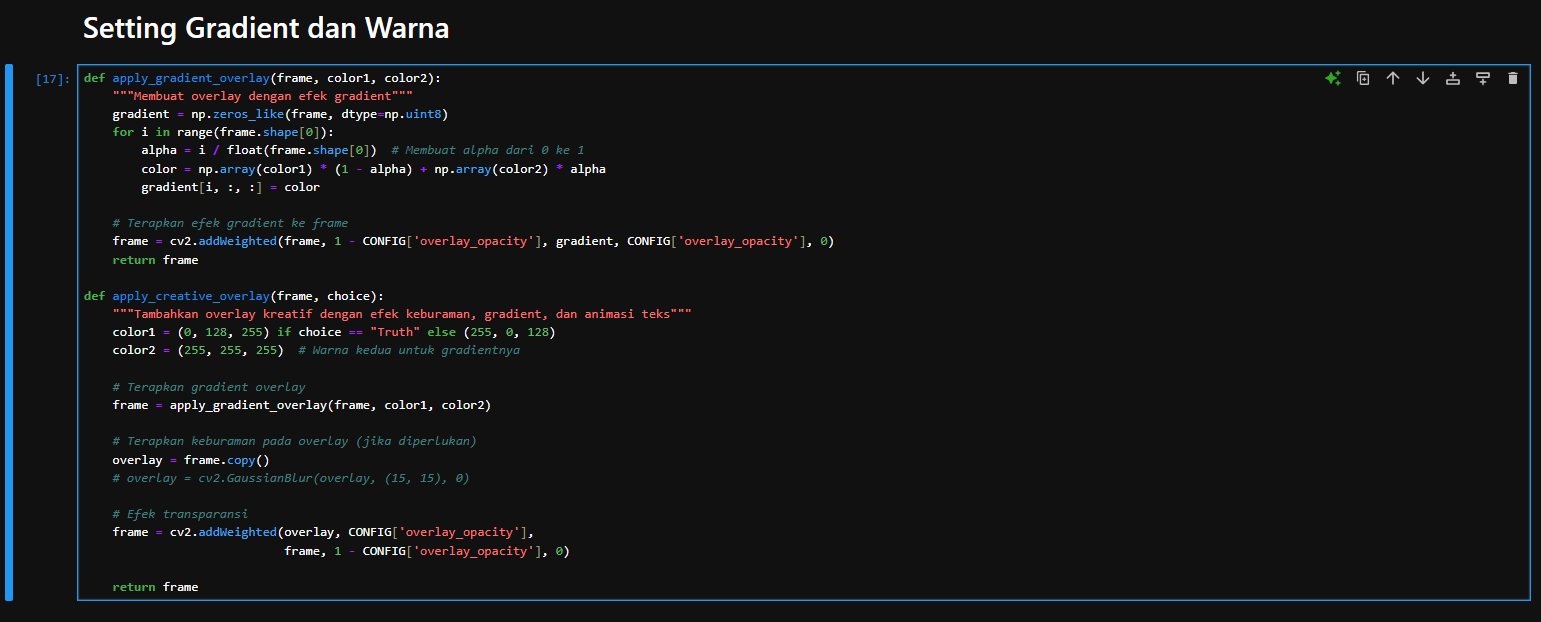
\includegraphics[width=0.8\textwidth]{6.png} % Sesuaikan nama file gambar
    \caption{Kode Program 6}
    \label{fig:6}
\end{figure}

\textbf{Fungsi apply\_gradient\_overlay}

Fungsi ini membuat efek \textbf{gradient} yang halus pada frame video dengan mencampurkan dua warna yang ditentukan (color1 dan color2).

\textbf{Penjelasan:}
\begin{enumerate}
    \item gradient = np.zeros\_like(frame, dtype=np.uint8):  
    
    Membuat sebuah array kosong yang memiliki ukuran yang sama dengan frame (gambar yang ditangkap dari kamera), dan tipe datanya adalah uint8, yang memungkinkan kita untuk bekerja dengan warna dalam format 8-bit.
    \item for i in range(frame.shape[0]):  
    
Fungsi ini mengiterasi sepanjang tinggi gambar (frame.shape[0]), untuk menerapkan gradien vertikal. Gradien akan bergerak dari color1 di bagian atas ke color2 di bagian bawah gambar.
    \item alpha = i / float(frame.shape[0]):  
    
    Menentukan nilai alpha (transparansi) untuk setiap baris vertikal. Nilai alpha berkisar antara 0 (untuk bagian atas gambar) hingga 1 (untuk bagian bawah gambar). Ini memungkinkan transisi yang halus antara dua warna.
    \item color = np.array(color1) * (1 - alpha) + np.array(color2) * alpha: 
    
    Mencampur kedua warna (color1 dan color2) berdasarkan nilai alpha. Semakin tinggi nilai alpha (semakin ke bawah gambar), semakin dominan warna kedua (color2), dan sebaliknya.
    \item gradient[i, :, :] = color:  
    
    Menerapkan warna yang dihitung pada setiap baris vertikal dari gambar.
    \item frame = cv2.addWeighted(frame, 1 - CONFIG['overlay\_opacity'], gradient, CONFIG['overlay\_opacity'], 0): 
    \begin{itemize}
        \item Menggabungkan gradient yang telah dibuat dengan frame video asli menggunakan fungsi cv2.addWeighted(). Ini menciptakan efek transparansi dengan mengatur overlay\_opacity (seberapa transparan efek gradient yang diterapkan).
        \item 1 - CONFIG['overlay\_opacity'] mengontrol tingkat transparansi gambar asli, dan CONFIG['overlay\_opacity'] mengontrol transparansi gradient.
    \end{itemize}
\end{enumerate}

\textbf{Return:}

Fungsi ini mengembalikan frame dengan efek gradient yang diterapkan di atasnya.

\textbf{Fungsi apply\_creative\_overlay  }

Fungsi ini menambahkan overlay kreatif dengan berbagai efek, termasuk \textbf{gradient}, \textbf{keburaman}, dan \textbf{transparansi}, untuk menambah daya tarik visual berdasarkan pilihan permainan (Truth atau Dare).

\textbf{Penjelasan:}
\begin{enumerate}
    \item color1 = (0, 128, 255) if choice == "Truth" else (255, 0, 128): 
    
    Menentukan warna pertama untuk gradient berdasarkan pilihan pemain. Jika pemain memilih Truth, warna pertama adalah oranye ((0, 128, 255)); jika pemain memilih Dare, warna pertama adalah merah muda ((255, 0, 128)).
    \item color2 = (255, 255, 255): 

    Warna kedua untuk gradient adalah putih ((255, 255, 255)).
    \item frame = apply\_gradient\_overlay(frame, color1, color2):  
    
    Fungsi apply\_gradient\_overlay dipanggil untuk menerapkan efek gradient pada frame dengan warna yang ditentukan oleh pilihan pemain.
    \item overlay = frame.copy():  
    
    Membuat salinan dari frame yang telah dimodifikasi untuk memungkinkan penerapan efek keburaman (blur) hanya pada overlay, tanpa mengubah frame asli.
    \item frame = cv2.addWeighted(overlay, CONFIG['overlay\_opacity'], frame, 1 - CONFIG['overlay\_opacity'], 0):  

    Menggabungkan overlay yang telah diblur (atau tidak) dengan frame video menggunakan transparansi yang ditentukan oleh overlay\_opacity. Ini akan menciptakan efek visual dengan transparansi untuk overlay yang diterapkan.
\end{enumerate}

\textbf{Return:}  
Fungsi ini mengembalikan frame yang telah dimodifikasi dengan overlay kreatif yang mencakup efek gradient, keburaman (jika diaktifkan), dan transparansi.

Penggunaan dalam Program:  
apply\_gradient\_overlay digunakan untuk menambahkan efek gradient vertikal yang lembut antara dua warna ke frame video.  
apply\_creative\_overlay digunakan untuk menambahkan overlay yang lebih kreatif, yang tidak hanya mencakup gradient, tetapi juga keburaman dan efek transparansi, berdasarkan pilihan permainan (Truth atau Dare).

\begin{figure}[H]
    \centering
    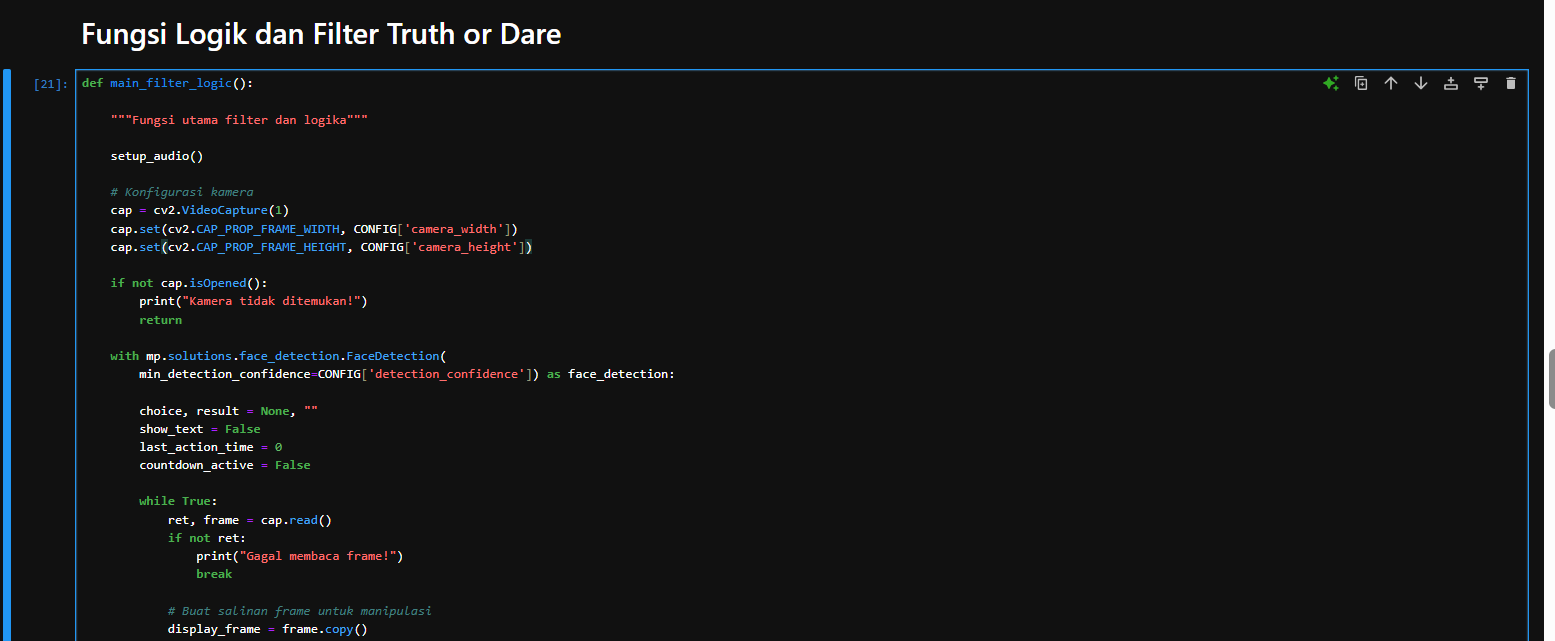
\includegraphics[width=0.8\textwidth]{7.png} % Sesuaikan nama file gambar
    \caption{Kode Program 7}
    \label{fig:7}
\end{figure}

\begin{figure}[H]
    \centering
    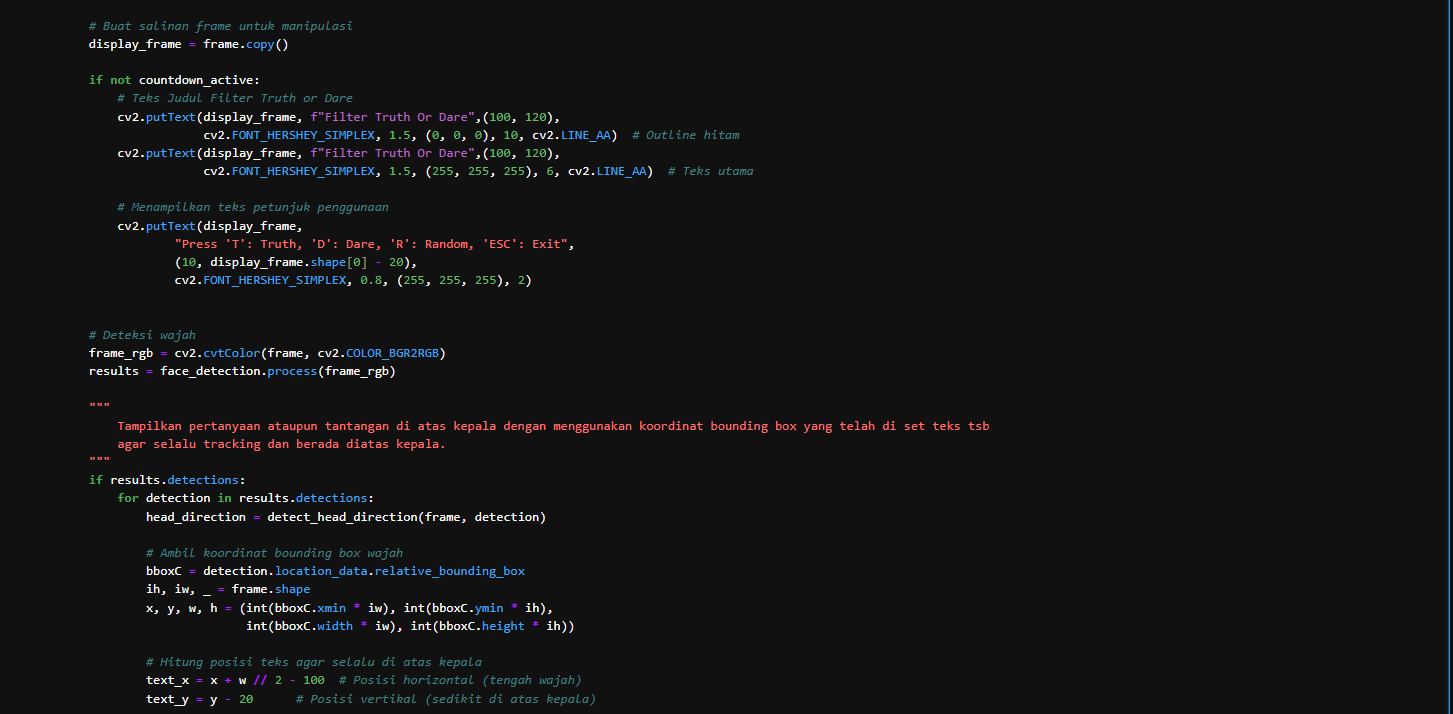
\includegraphics[width=0.8\textwidth]{8.png} % Sesuaikan nama file gambar
    \caption{Kode Program 8}
    \label{fig:8}
\end{figure}

\begin{figure}[H]
    \centering
    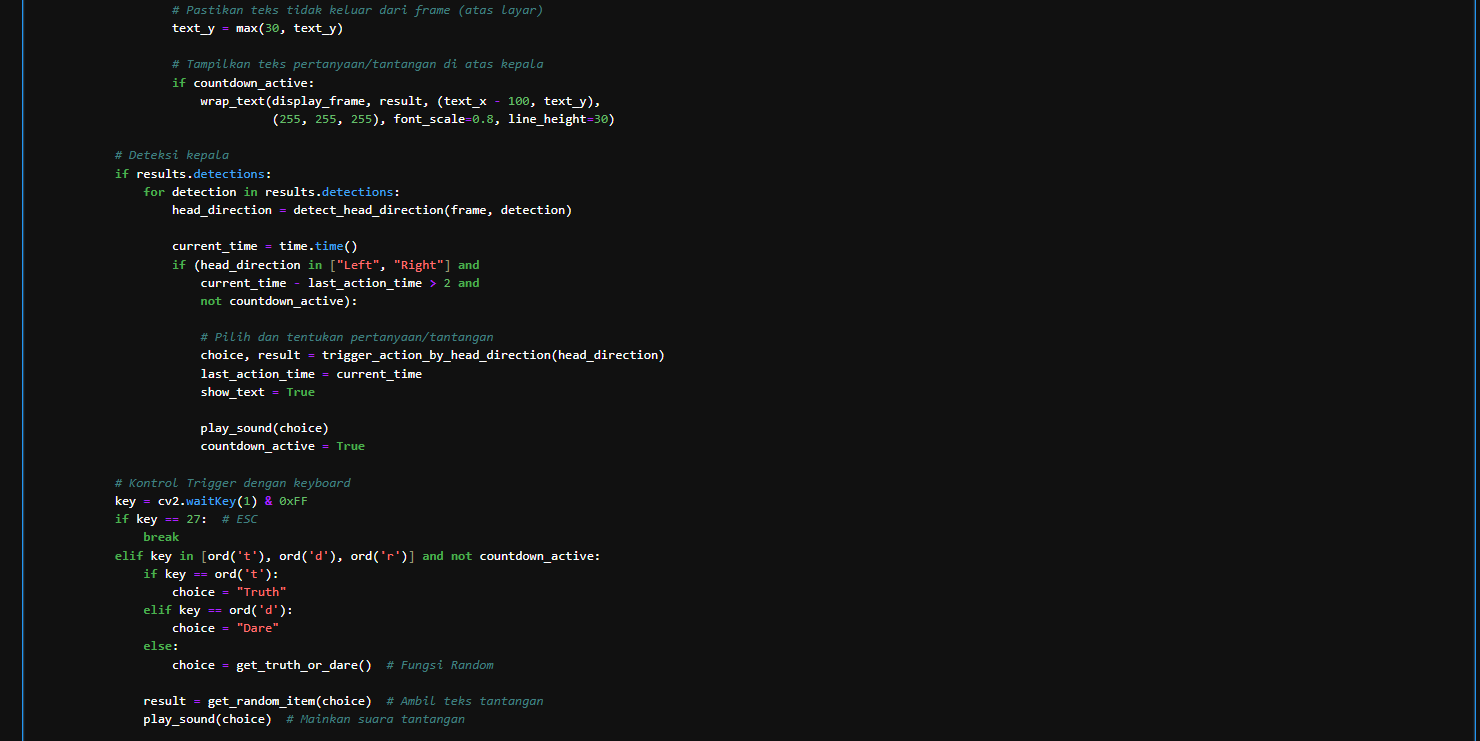
\includegraphics[width=0.8\textwidth]{9.png} % Sesuaikan nama file gambar
    \caption{Kode Program 9}
    \label{fig:9}
\end{figure}

\begin{figure}[H]
    \centering
    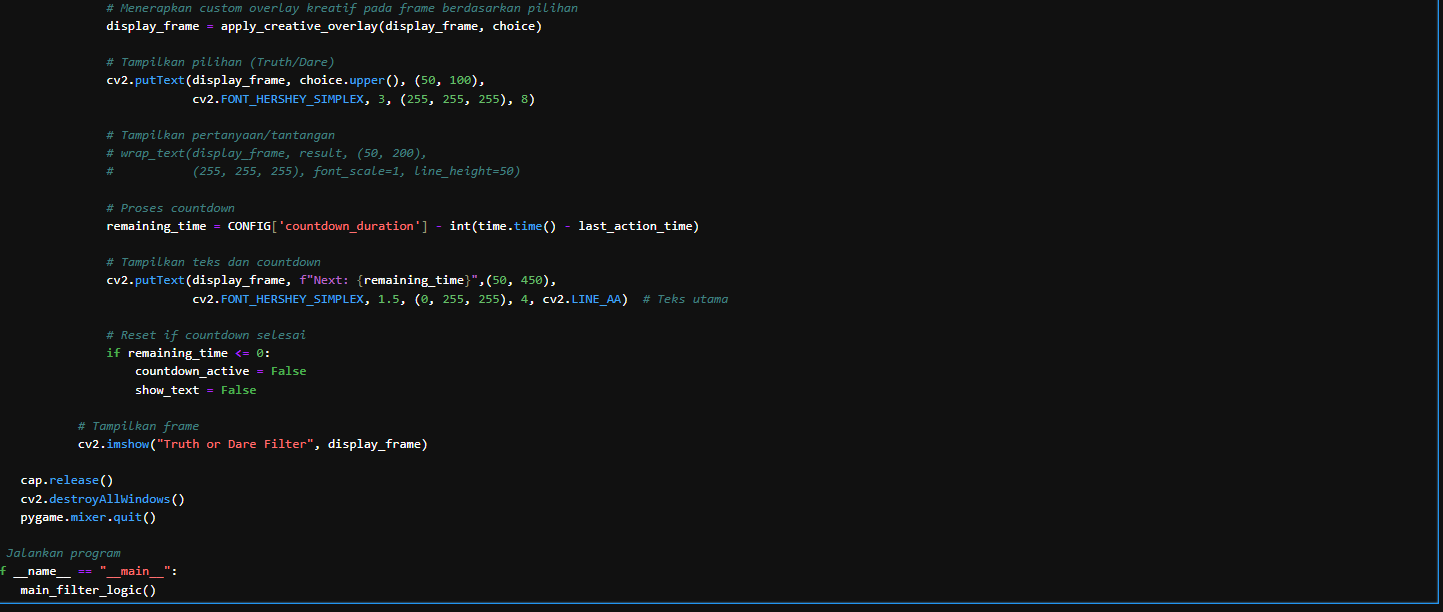
\includegraphics[width=0.8\textwidth]{10.png} % Sesuaikan nama file gambar
    \caption{Kode Program 10}
    \label{fig:10}
\end{figure}

\textbf{1. Setup Audio}  

setup\_audio(): Fungsi ini menginisialisasi pemutaran audio. Kemungkinan ini digunakan untuk suara latar atau efek suara yang digunakan dalam permainan, seperti suara yang diputar ketika pilihan (Truth/Dare) dipilih.

\textbf{2. Konfigurasi Kamera  }

Program ini menginisialisasi kamera menggunakan cv2.VideoCapture(1) dan mengatur resolusi berdasarkan nilai konfigurasi di CONFIG.  
Jika kamera tidak ditemukan atau gagal dibuka, pesan kesalahan akan ditampilkan.

\textbf{3. Deteksi Wajah dengan Mediapipe}

mp.solutions.face\_detection.FaceDetection digunakan untuk deteksi wajah, dengan ambang batas kepercayaan minimum yang diatur oleh CONFIG['detection\_confidence'].  

Untuk setiap wajah yang terdeteksi, program memproses koordinat bounding box (bboxC) dan mendeteksi arah kepala berdasarkan posisi relatif wajah dalam frame.

\textbf{4. Loop Utama Permainan }

\textbf{Menampilkan teks:} 

Judul "Filter Truth Or Dare" ditampilkan dengan font besar di bagian atas frame. 

Instruksi cara bermain juga ditampilkan di bagian bawah frame (misalnya, "Tekan 'T' untuk Truth, 'D' untuk Dare").  

\textbf{Deteksi Arah Kepala:}

Jika kepala pemain bergerak ke kiri atau kanan, permainan mengenali arah ini dan memicu aksi (Truth atau Dare).

detect\_head\_direction: Menentukan apakah kepala pemain menghadap kiri, kanan, atau netral.  

\textbf{Input Keyboard:}  

Pemain dapat memilih pilihan secara manual dengan menekan 'T' untuk Truth, 'D' untuk Dare, atau 'R' untuk pilihan acak.  

Setelah pilihan dibuat, aksi yang sesuai dipicu, dan penghitung mundur dimulai.

\textbf{5. Logika Countdown  }

Begitu pilihan dibuat (baik oleh arah kepala atau input keyboard), timer countdown dimulai, dan tantangan truth atau dare ditampilkan di atas kepala pemain.  

Timer menghitung mundur hingga aksi berikutnya dipicu. Ketika countdown selesai, permainan direset, dan pemain dapat memilih lagi.

\textbf{6. Pembungkusan Teks }

wrap\_text() adalah fungsi kustom (tidak disertakan dalam kode) yang membungkus teks agar dapat ditampilkan di beberapa baris jika teks tersebut tidak cukup untuk satu baris.  

Fungsi ini digunakan untuk menampilkan tantangan (pertanyaan truth atau dare) di posisi yang dihitung di atas kepala pemain.

\textbf{7. Creative Overlay  }

apply\_creative\_overlay() menambahkan overlay visual kustom berdasarkan pilihan pemain Truth atau Dare.  

Efek gradien diterapkan dengan warna yang bergantung pada pilihan (Truth = oranye, Dare = merah muda).  

Overlay memiliki efek transparansi yang dapat berubah berdasarkan status countdown.

\textbf{8. Tampilan Frame dan Pembersihan } 

Setelah memproses frame dan menambahkan efek atau teks, frame ditampilkan menggunakan cv2.imshow().  

Loop terus berjalan hingga pengguna menekan tombol ESC untuk keluar, setelah itu sumber daya dibebaskan, dan jendela ditutup.


\begin{figure}[H]
    \centering
    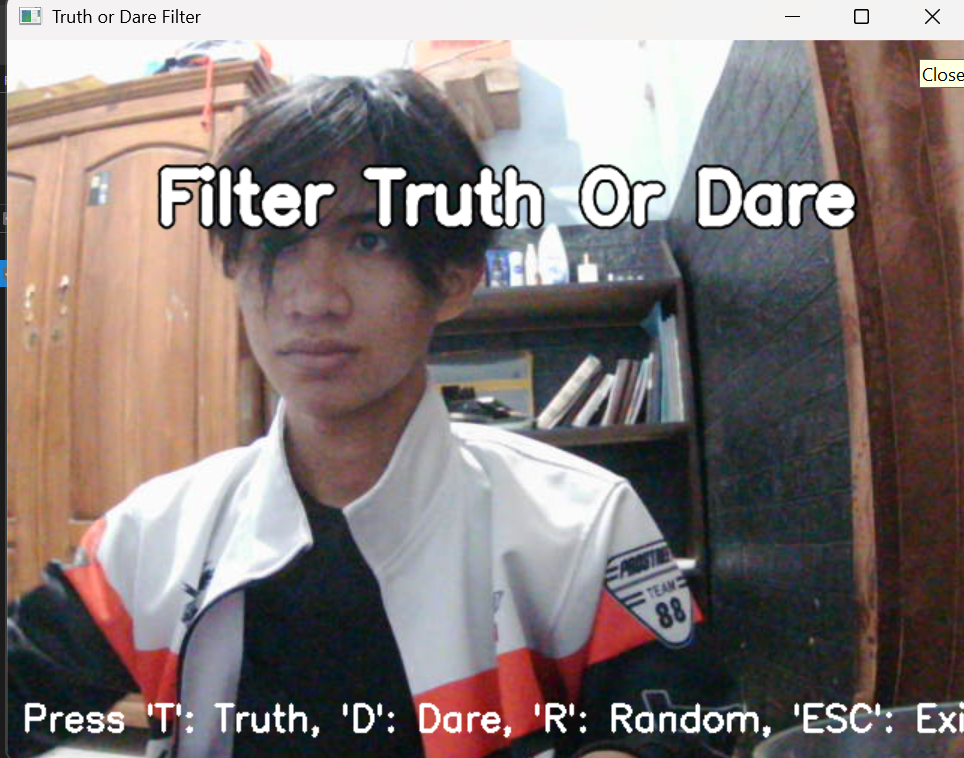
\includegraphics[width=0.8\textwidth]{11.png} % Sesuaikan nama file gambar
    \caption{Hasil 1}
    \label{fig:11}
\end{figure}

\begin{figure}[H]
    \centering
    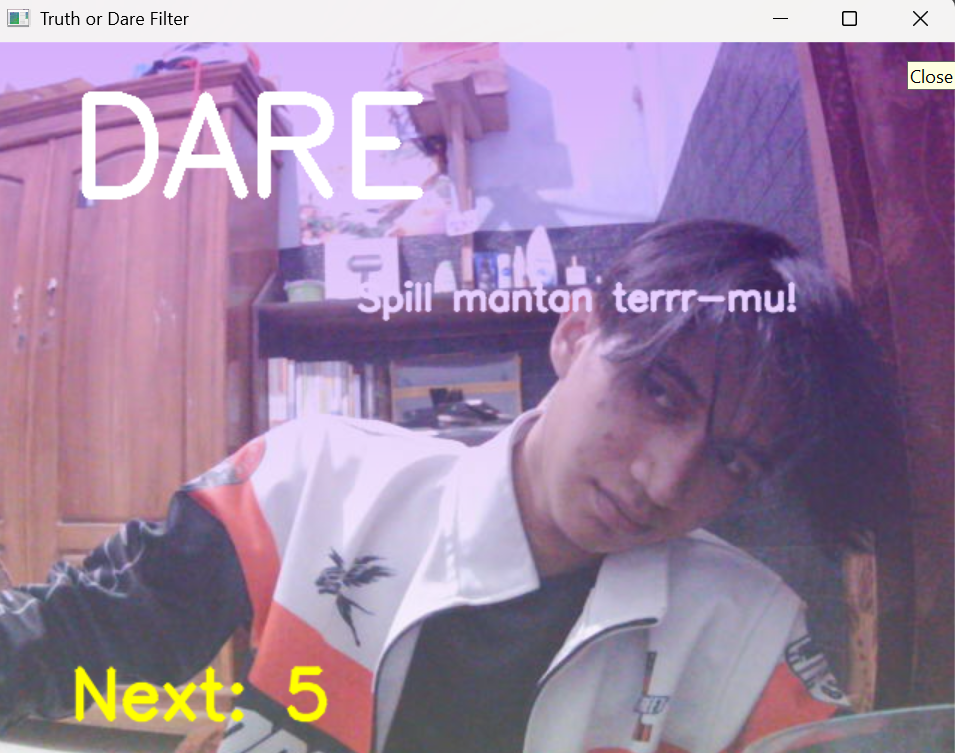
\includegraphics[width=0.8\textwidth]{12.png} % Sesuaikan nama file gambar
    \caption{Hasil 2}
    \label{fig:12}
\end{figure}

\begin{figure}[H]
    \centering
    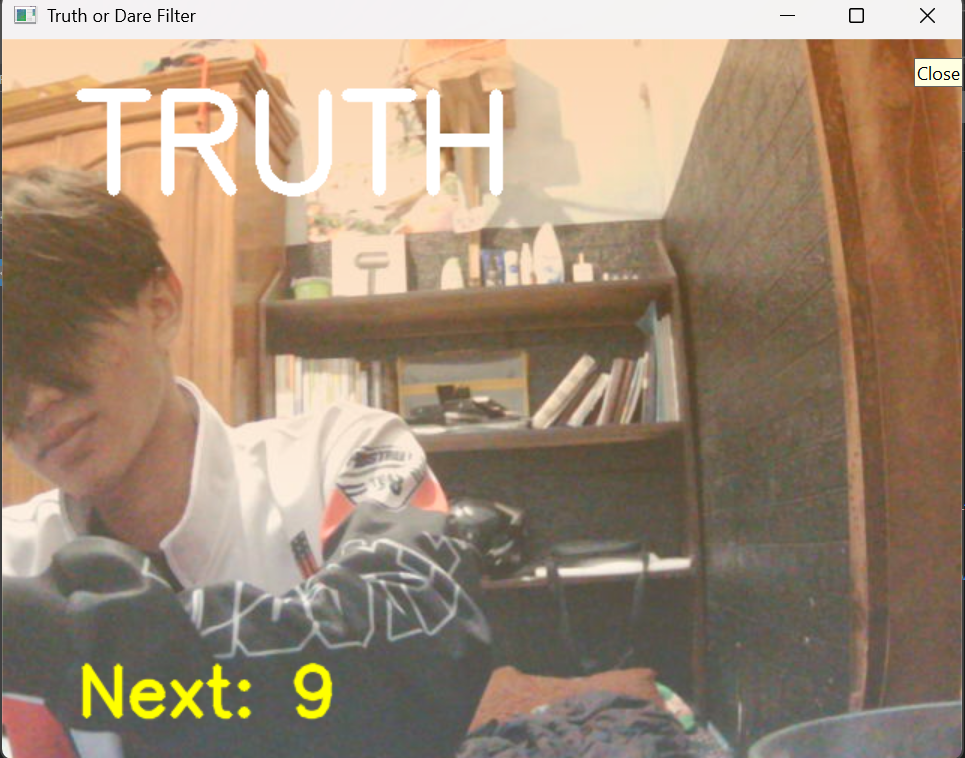
\includegraphics[width=0.8\textwidth]{13.png} % Sesuaikan nama file gambar
    \caption{Hasil 3}
    \label{fig:13}
\end{figure}

\newpage
\section{Kesimpulan dan Saran}
\subsection{Kesimpulan}
Berdasarkan hasil implementasi dan pengujian, program "Filter Truth or Dare" berhasil meningkatkan pengalaman bermain yang interaktif melalui penggunaan teknologi pelacakan wajah. Pengguna merasa lebih terlibat dalam permainan karena adanya elemen interaktif yang memberikan tantangan atau pertanyaan secara acak berdasarkan gerakan wajah. Program ini juga mampu menciptakan dampak positif terhadap interaksi sosial dengan meningkatkan keterlibatan antar pemain. Hiburan yang ditawarkan program ini tidak hanya mendukung pengalaman bermain yang menyenangkan tetapi juga memperkuat hubungan sosial antar pengguna.

\subsection{Saran}
Meskipun program "Filter Truth or Dare" berhasil meningkatkan pengalaman bermain yang interaktif, beberapa perbaikan dan pengembangan dapat dilakukan untuk lebih mengoptimalkan sistem ini. Pertama, peningkatan akurasi deteksi wajah dan arah kepala dalam berbagai kondisi pencahayaan dapat membantu meningkatkan pengalaman pengguna, terutama bagi pemain yang berada di lingkungan dengan pencahayaan yang kurang ideal. Selain itu, menambahkan lebih banyak variasi dalam pertanyaan atau tantangan Truth dan Dare yang tersedia dapat memberikan pengalaman yang lebih menarik dan tidak monoton. Program juga dapat diperluas dengan menambahkan opsi untuk menyesuaikan efek visual dan audio, sehingga pemain dapat lebih mengontrol pengalaman permainan mereka. Untuk mendukung interaksi sosial yang lebih baik, pengembangan fitur multiplayer atau kemampuan berbagi hasil permainan secara langsung dapat menjadi tambahan yang menarik. Terakhir, pengujian lebih lanjut pada berbagai perangkat dengan spesifikasi berbeda diperlukan untuk memastikan kinerja yang optimal pada berbagai platform. Dengan melakukan perbaikan ini, program dapat memberikan pengalaman yang lebih imersif dan menyenangkan bagi lebih banyak pengguna.\dots

\newpage
\bibliographystyle{IEEEtran}
\bibliography{Referensi}
[1] 
Y. Zhang, X. Wang, and L. Zhang, "Face Tracking Using Deep Learning Techniques," IEEE Transactions on Image Processing, vol. 29, pp. 1234-1245, 2020.

[2] 
Y. Liu and H. Wang, "Augmented Reality in Social Applications: A Study on User Engagement," Journal of Augmented and Virtual Reality, vol. 5, no. 2, pp. 45-58, 2021.

[3] 
J. Kim, S. Lee, and M. Park, "User Experience Evaluation of Face Filters in Interactive Games," International Journal of Human-Computer Interaction, vol. 35, no. 3, pp. 215-230, 2019.

[4] 
G. van Rossum and F. L. Drake, Python 3 Reference Manual, CreateSpace, 2011.

[5] 
A. Stolwijk, Solution Concepts in Cooperative Game Theory, 2010. 

[6] 
"PENGUJIAN BLACK BOX TESTING PADA APLIKASI ACTION & STRATEGY BERBASIS ANDROID DENGAN TEKNOLOGI PHONEGAP," Jurnal String (Satuan Tulisan Riset dan Inovasi Teknologi), vol. 3, no. 2, pp. 206-210, 2018. 

[7] 
S. R. Fadillah, E. M. A. Jonemaro and W. S. Wardhono, "Pengembangan Gim Edukasi Matematika Dasar berbasis Android," Jurnal Pengembangan Teknologi Informasi dan Ilmu Komputer, vol. 5, no. 3, pp. 1142-1148, 2021. 


\end{document}
